\begin{center}
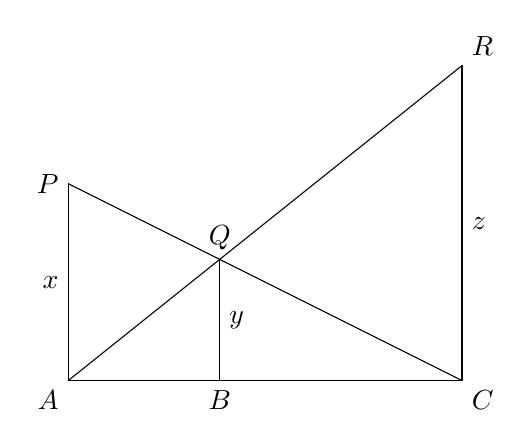
\begin{tikzpicture}[scale=1.0, line cap=round, line join=round]

    % Coordinates
    \coordinate (A) at (0,0);
    \coordinate (C) at (5,0);
    \coordinate (P) at (0,2.5);
    \coordinate (R) at (5,4);
    
    % Intersection of AR and PC
    \coordinate (Q) at (1.923,1.538);
    \coordinate (B) at (1.923,0);

    % Base AC
    \draw (A)--(C);

    % Perpendicular lines
    \draw (A)--(P);
    \draw (B)--(Q);
    \draw (C)--(R);

    % Slanting lines
    \draw (A)--(R);
    \draw (P)--(C);

    % Point labels
    \node[below left]  at (A) {$A$};
    \node[below]       at (B) {$B$};
    \node[below right] at (C) {$C$};
    \node[left]        at (P) {$P$};
    \node[above]       at (Q) {$Q$};
    \node[above right] at (R) {$R$};

    % Length labels
    \node[left] at (0,1.25) {$x$};
    \node[right] at (1.923,0.77) {$y$};
    \node[right] at (5,2) {$z$};

\end{tikzpicture}
\end{center}
